\lecture{9}{24. Februar 2025}{Static Loading and Fracture}

\exercise{8.1} Estimate the theoretical fracture strength of a brittle material if it is known that fracture occurs by the propagation of an elliptically shaped surface crack of length \qty{0,5}{mm} and a tip radius of curvature of \qty{5e-3}{mm}, when a stress of \qty{1035}{MPa} is applied.
\bigbreak
We know that fracturing happens when fractures propagate. The critical stress for a crack to propagate is given by the formula for the amplification of stress at flaws:
\[ 
\sigma_m = 2\sigma_0 \sqrt{\frac{a}{\rho_t}}
.\]
By plugging in known values we get
\[ 
\sigma_m = 2 \cdot \qty{1035}{MPa} \cdot \sqrt{\frac{\qty{0,25}{mm}}{\qty{5e-3}{mm}}} = \qty{14640}{MPa} 
.\]



\exercise{8.3} A specimen of a 4340 steel alloy with a plane strain fracture toughness of \qty{54,8}{\MPa.\sqrt{m}} is exposed to a stress of \qty{1030}{MPa}. Will this specimen experience fracture if the largest surface crack is \qty{0,5}{mm} long? Why or why not? Assume that the parameter $Y$ has a value of \num{1,0}.
\bigbreak
The fracture toughness is given by the formula
\[ 
K_{Ic} = Y \sigma_{c} \sqrt{\pi a}
.\]
Using this we can calculate the applied stress intensity factor $K_{\mathrm{applied}}$ as
\[ 
  K_{\mathrm{applied}} = 1 \cdot \qty{1030}{MPa} \sqrt{\pi \cdot \qty{0,5}{mm}} = \qty{40,82}{\MPa.\sqrt{m}} 
.\]
As $K_{\mathrm{applied}} = \qty{40,82}{\MPa.\sqrt{m}} < \qty{54,8}{\MPa.\sqrt{m}} = K_{Ic}$ the steel should be able to withstand the stress.



\exercise{8.7} The following tabulated data were gathered from a series of Charpy impact tests on a tempered 4340 steel alloy. 
\begin{table}[ht]
\centering
\begin{tabular}{|l|l|}
\hline
\textbf{Temperature (\unit{\celsius})} & \textbf{Impact Energy (\unit{J})} \\ \hline
\textit{$0$}                           & $105$                             \\ \hline
\textit{$-25$}                         & $104$                             \\ \hline
\textit{$-50$}                         & $103$                             \\ \hline
\textit{$-75$}                         & $97$                              \\ \hline
$-100$                                 & $63$                              \\ \hline
$-113$                                 & $40$                              \\ \hline
$-125$                                 & $34$                              \\ \hline
$-150$                                 & $28$                              \\ \hline
$-175$                                 & $25$                              \\ \hline
$-200$                                 & $24$                              \\ \hline
\end{tabular}
\end{table}

\paragraph{(a)} Plot the data as impact energy versus temperature.
\bigbreak
\begin{figure} [ht]
  \centering
  \caption{Impact energy vs. temperature}
  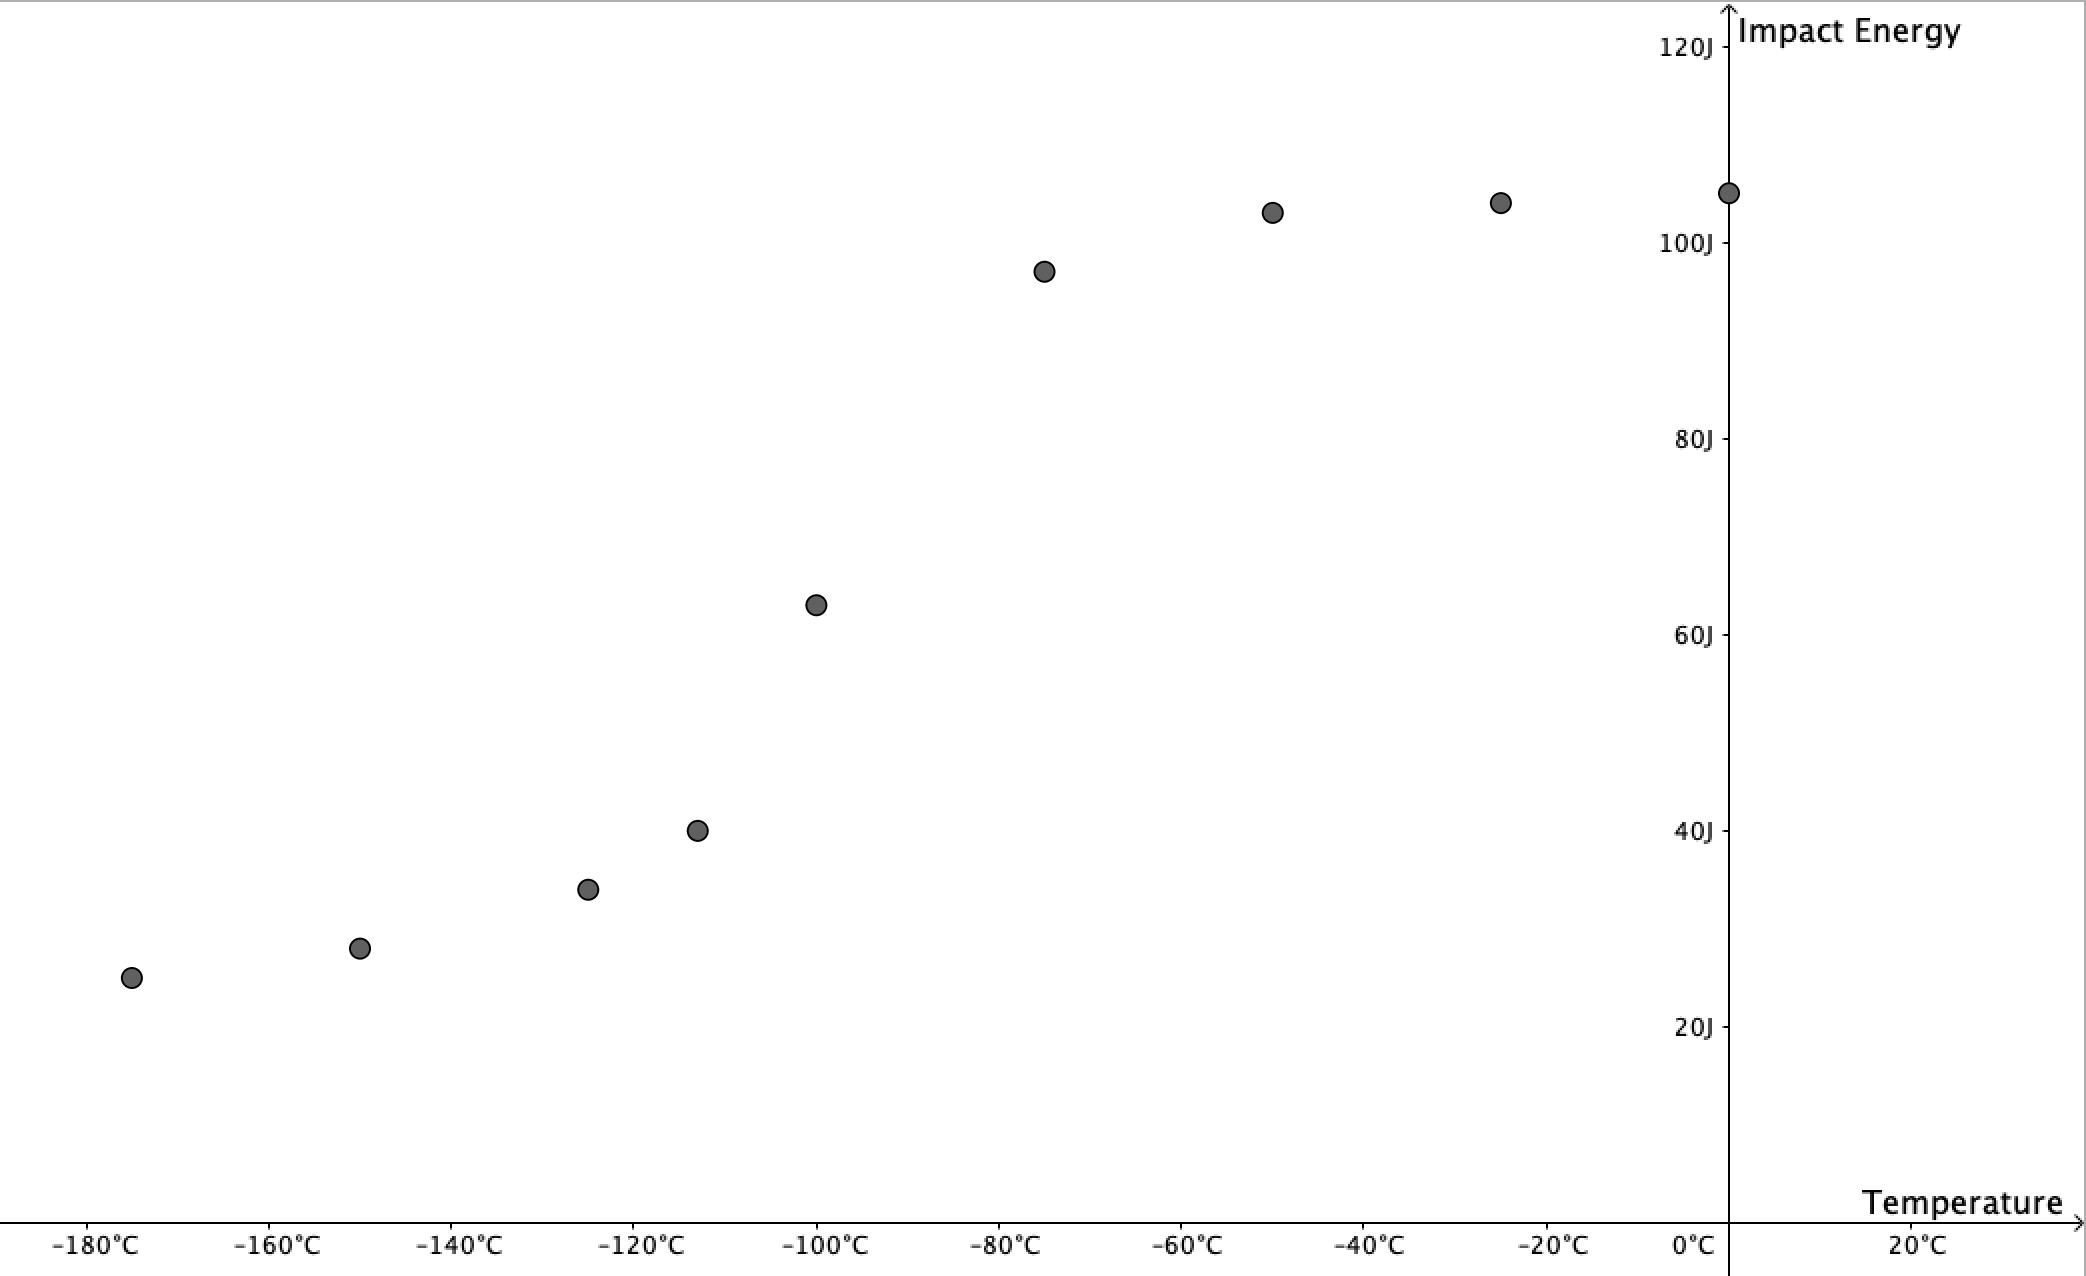
\includegraphics[width=0.5\linewidth]{./figures/f9_1.png}
  \label{fig:f9_1}
\end{figure}

\paragraph{(b)} Determine a ductile-to-brittle transition temperature as the temperature corresponding to the average of the maximum and minimum impact energies.
\bigbreak
The maximum impact energy is \qty{105}{J} and the minimum is \qty{24}{J}. The average of these two values is
\[ 
\frac{\qty{105}{J} + \qty{24}{J}}{2} = \qty{64,5}{J} 
.\]
This impact energy is a little above the \qty{-100}{\celsius} mark so a reasonable approximation would be something like \qty{-97}{\celsius}.

\paragraph{(c)} Determine a ductile-to-brittle transition temperature as the temperature at which the impact energy is \qty{50}{J}.
\bigbreak
The impact energy is \qty{50}{J} somewhere between the temperatures of \qty{-100}{\celsius} and \qty{-113}{\celsius}. By linear interpolation the impact energy is \qty{50}{J} roughly at \qty{-105}{\celsius}.
